%%% CSE 4316 Project Charter - WORKED EXAMPLE (Mobile App + IoT). Follows ISO/IEC/IEEE 16326:2019.
\documentclass[11pt,letterpaper]{article}
\usepackage[margin=1.0in]{geometry}
\usepackage[T1]{fontenc}\usepackage[bitstream-charter]{mathdesign}\usepackage[latin1]{inputenc}
\usepackage{amsmath}\usepackage{xcolor}\usepackage{cite}\usepackage{hyphenat}
\usepackage{graphicx}\usepackage{float}\usepackage{subfigure}\usepackage{sectsty}
\usepackage[compact]{titlesec}\usepackage[tablegrid]{vhistory}\usepackage{longtable}
\allsectionsfont{\color{accentcolor}\scshape\selectfont}
\definecolor{accentcolor}{rgb}{0.0,0.0,0.5}
\newcommand{\teamname}{Team Nimbus}
\newcommand{\productname}{AquaGuard Smart Water-Leak Monitor}
\newcommand{\coursename}{CSE 4316: Senior Design I}
\newcommand{\semester}{Fall 2026}
\newcommand{\docname}{Project Charter}
\newcommand{\department}{Department of Computer Science \& Engineering}
\newcommand{\university}{The University of Texas at Arlington}
\newcommand{\authors}{Alan Turing \\ Grace Hopper \\ John Von Neumann \\ Ada Lovelace \\ Charles Babbage}
\usepackage{fancyhdr}\pagestyle{fancy}\usepackage{lastpage}
\lhead{}\chead{}\rhead{}\lfoot{\footnotesize \teamname \ - \semester}\cfoot{}
\rfoot{\footnotesize page \thepage\ of \pageref{LastPage}}
\renewcommand{\headrulewidth}{0.0pt}\renewcommand{\footrulewidth}{0.4pt}
\usepackage[runin]{abstract}\abslabeldelim{\quad}\setlength{\abstitleskip}{-10pt}
\renewcommand{\abstractname}{}\renewcommand{\abstracttextfont}{\color{accentcolor} \small \slshape}

\begin{document}
{\centering \huge \color{accentcolor} \sc \textbf{\department \\ \university} \par}
\vspace{1 in}
{\centering \huge \color{accentcolor} \sc \textbf{\docname \\ \coursename \\ \semester} \par}
\vspace{0.5 in}
\begin{figure}[h!]\centering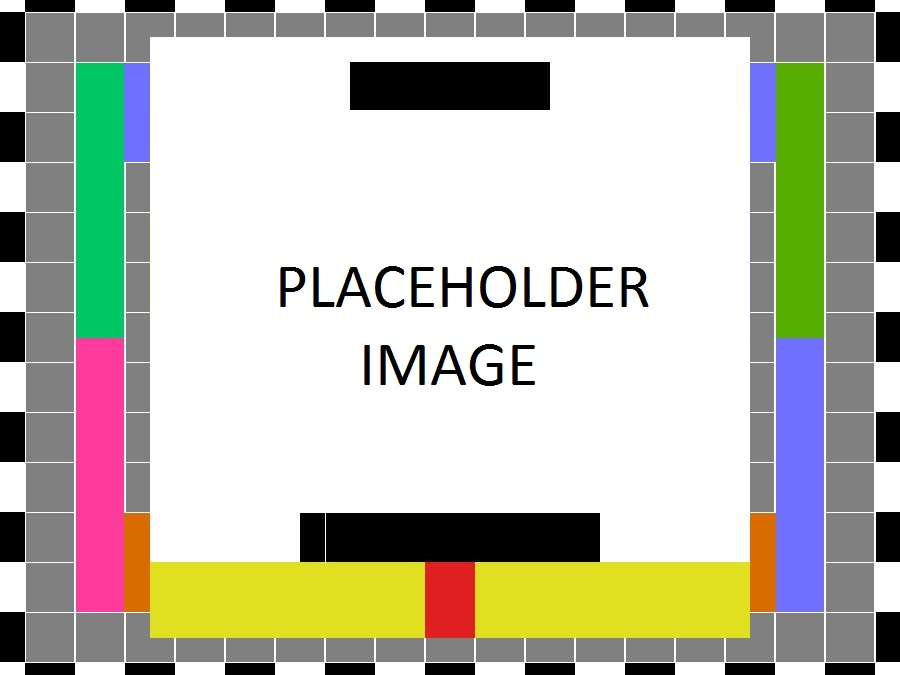
\includegraphics[width=0.60\textwidth]{images/test_image}\end{figure}
\vspace{0.5 in}
{\centering \huge \color{accentcolor} \sc \textbf{\teamname \\ \productname} \par}
\vspace{0.5 in}{\centering \large \sc \textbf{\authors} \par}
\newpage
\begin{versionhistory}
  \vhEntry{0.1}{09.02.2026}{GH}{document creation}
  \vhEntry{1.0}{09.15.2026}{AT|GH|CB}{official release}
\end{versionhistory}
\newpage\tableofcontents\newpage

\section{Problem Statement}
Household water leaks under sinks and behind appliances often go unnoticed for hours
or days, causing expensive damage and wasted water. Homeowners have no early warning
until they see or smell the damage. What is needed is an inexpensive way to detect
leaks the moment they start and alert the homeowner immediately, wherever they are.

\section{Methodology}
Team Nimbus will build \productname, a small battery-powered sensor device that
detects moisture and abnormal flow under a sink and communicates over Bluetooth Low
Energy (BLE) with a companion phone app. The app pairs and configures the device,
raises immediate alerts on a leak, and shows event history. In short: we are
building a small sensor plus a phone app that warns you the instant a leak starts.

\section{Value Proposition}
For homeowners, AquaGuard turns costly, late-discovered water damage into an early,
actionable alert, at a fraction of the cost of professional leak systems. For the
university, the project exercises the full IoT stack --- embedded firmware, BLE
protocol design, a cross-platform mobile app, and cloud push notifications.

\section{Development Milestones}
\begin{itemize}
  \item Project Charter first draft - September 2026
  \item System Requirements Specification - October 2026
  \item Architectural Design Specification - November 2026
  \item Demonstration of BLE pairing \& live sensor read - December 2026
  \item Detailed Design Specification - February 2027
  \item Demonstration of on-device leak detection \& local alert - March 2027
  \item Demonstration of remote push notification - April 2027
  \item CoE Innovation Day poster presentation - April 2027
  \item Final Project Demonstration (end-to-end leak alert) - May 2027
\end{itemize}
\newpage

\section{Background}
The project is team-initiated with an industry mentor from a home-automation startup
acting as advisor. There is no paying customer; the target user is a general
homeowner. Requirements were gathered from mentor interviews and a survey of
commercial leak sensors.

\section{Related Work}
Commercial leak sensors (e.g. Wi-Fi water sensors) exist \cite{Rubin2012} but many
require a hub, mains power, or a subscription. AquaGuard targets a low-cost,
battery-powered, hub-free BLE device with an open companion app. (Add $\geq$5 IEEE
references in the final version.)

\section{System Overview}
The sensor device (moisture pad + flow sensor + microcontroller with BLE) advertises
readings and events. The phone app (BLE central) pairs with the device, configures
thresholds, alerts locally on a leak, and forwards events to a lightweight cloud
backend that delivers push notifications when the phone is away. See the ADS for the
three-layer design.

\section{Project Management Approach}
Iterative Scrum \cite{Rubin2012, SchwaberSutherland2020} per ISO/IEC/IEEE 16326:2019
\cite{ISO16326} within ISO/IEC/IEEE 12207:2017 \cite{ISO12207} and 15288:2023
\cite{ISO15288} (the latter covering the hardware element). Two-week sprints;
estimation in task-hours; progress by burndown and requirement/test coverage. Git
with tagged releases; firmware and app versioned together.

\section{Roles \& Responsibilities}
Advisor: home-automation mentor. Product Owner: Grace Hopper. Scrum Master: Alan
Turing. Firmware/hardware: Charles Babbage; BLE protocol: John Von Neumann; Mobile
app: Ada Lovelace; Cloud/push: Grace Hopper; Integration/test: Alan Turing.

\section{Cost Proposal}
Major expenses: microcontroller + BLE module, moisture/flow sensors, battery and
enclosure (3D-printed), and a small cloud allocation for push. Funded by the default
CSE stipend. Largest line item is the sensor + BLE module across several prototype
revisions.

\section{Facilities \& Equipment}
Senior Design lab (soldering, 3D printing, bench supply), personal iOS/Android test
phones, and a controlled water test rig (a tray and dripper) by the 3rd sprint.

\section{Assumptions}
\begin{itemize}
  \item Team members can test on both a recent iOS and a recent Android phone.
  \item A controlled water test rig will be available by the 3rd sprint.
  \item A free-tier push-notification service will meet demo volume.
  \item BLE range under a cabinet ($\leq$5\,m through one wall) is sufficient.
  \item The device runs $\geq$6 months on one coin/AA battery set.
\end{itemize}

\section{Constraints}
\begin{itemize}
  \item Final demonstration must be completed by May 1st, 2027.
  \item Total development cost must not exceed \$800.
  \item The device must be battery-powered (no mains wiring).
  \item The app must run on current iOS and Android without app-store approval delays blocking the demo (use test/ad-hoc builds).
  \item Wireless design must comply with BLE (Bluetooth SIG) specifications.
\end{itemize}

\section{Risks}
\begin{table}[h]\resizebox{\textwidth}{!}{
\begin{tabular}{|l|l|l|l|}
\hline
\textbf{Risk description} & \textbf{Probability} & \textbf{Loss (days)} & \textbf{Exposure (days)} \\ \hline
BLE reliability/background behavior differs iOS vs Android & 0.50 & 12 & 6.0 \\ \hline
Battery life target hard to meet & 0.40 & 12 & 4.8 \\ \hline
Sensor false positives/negatives on real leaks & 0.40 & 10 & 4.0 \\ \hline
Push notification delivery when app backgrounded & 0.30 & 8 & 2.4 \\ \hline
Enclosure waterproofing revisions & 0.25 & 8 & 2.0 \\ \hline
\end{tabular}}
\caption{Highest-exposure project risks}
\end{table}

\section{Documentation \& Reporting}
Documentation deliverables in Git, released at their planning sprints; recurring
sprint artifacts and engineering notebooks each sprint. Closeout: sensor prototype +
app, poster, public web page, demo video, documented source (MIT), firmware
sources, enclosure CAD (STL/STEP), wiring schematic, app build/deploy instructions,
and a user setup guide.

\bibliographystyle{reference/IEEEtran_custom}
\bibliography{reference/refs}{}
\end{document}
